\documentclass[
  bibliography=totoc,     % Literatur im Inhaltsverzeichnis
  captions=tableheading,  % Tabellenüberschriften
  titlepage=firstiscover, % Titelseite ist Deckblatt
]{scrartcl}

% Paket float verbessern
\usepackage{scrhack}

% Warnung, falls nochmal kompiliert werden muss
\usepackage[aux]{rerunfilecheck}

% unverzichtbare Mathe-Befehle
\usepackage{amsmath}
% viele Mathe-Symbole
\usepackage{amssymb}
% Erweiterungen für amsmath
\usepackage{mathtools}

% Fonteinstellungen
\usepackage{fontspec}
% Latin Modern Fonts werden automatisch geladen
% Alternativ:
%\setromanfont{Libertinus Serif}
%\setsansfont{Libertinus Sans}
%\setmonofont{Libertinus Mono}
\recalctypearea % Wenn man andere Schriftarten gesetzt hat,
% sollte man das Seiten-Layout neu berechnen lassen

% deutsche Spracheinstellungen
\usepackage{polyglossia}
\setmainlanguage{german}
%test

\usepackage[
  math-style=ISO,    % ┐
  bold-style=ISO,    % │
  sans-style=italic, % │ ISO-Standard folgen
  nabla=upright,     % │
  partial=upright,   % ┘
  warnings-off={           % ┐
    mathtools-colon,       % │ unnötige Warnungen ausschalten
    mathtools-overbracket, % │
},                       % ┘
]{unicode-math}

% traditionelle Fonts für Mathematik
\setmathfont{Latin Modern Math}
% Alternativ:
%\setmathfont{Libertinus Math}

\setmathfont{XITS Math}[range={scr, bfscr}]
\setmathfont{XITS Math}[range={cal, bfcal}, StylisticSet=1]

% Zahlen und Einheiten
\usepackage[
locale=DE,                   % deutsche Einstellungen
separate-uncertainty=true,   % immer Fehler mit \pm
per-mode=symbol-or-fraction, % / in inline math, fraction in display math
]{siunitx}

% chemische Formeln
\usepackage[
version=4,
math-greek=default, % ┐ mit unicode-math zusammenarbeiten
text-greek=default, % ┘
]{mhchem}

% richtige Anführungszeichen
\usepackage[autostyle]{csquotes}

% schöne Brüche im Text
\usepackage{xfrac}

% Standardplatzierung für Floats einstellen
\usepackage{float}
\floatplacement{figure}{htbp}
\floatplacement{table}{htbp}

% Floats innerhalb einer Section halten
\usepackage[
section, % Floats innerhalb der Section halten
below,   % unterhalb der Section aber auf der selben Seite ist ok
]{placeins}

% Seite drehen für breite Tabellen: landscape Umgebung
\usepackage{pdflscape}

% Captions schöner machen.
\usepackage[
  labelfont=bf,        % Tabelle x: Abbildung y: ist jetzt fett
  font=small,          % Schrift etwas kleiner als Dokument
  width=0.9\textwidth, % maximale Breite einer Caption schmaler
]{caption}
% subfigure, subtable, subref
\usepackage{subcaption}

% Grafiken können eingebunden werden
\usepackage{graphicx}
% größere Variation von Dateinamen möglich
\usepackage{grffile}

% schöne Tabellen
\usepackage{booktabs}

% Verbesserungen am Schriftbild
\usepackage{microtype}

% Literaturverzeichnis
\usepackage[style=alphabetic,]{biblatex}
% Quellendatenbank
\addbibresource{lit.bib}
\addbibresource{programme.bib}

% Hyperlinks im Dokument
\usepackage[
  unicode,        % Unicode in PDF-Attributen erlauben
  pdfusetitle,    % Titel, Autoren und Datum als PDF-Attribute
  pdfcreator={},  % ┐ PDF-Attribute säubern
  pdfproducer={}, % ┘
]{hyperref}
% erweiterte Bookmarks im PDF
\usepackage{bookmark}

% Trennung von Wörtern mit Strichen
\usepackage[shortcuts]{extdash}

\title{V44: Röntgenreflektrometrie}
\author{
  Martin Schönfeld
  \texorpdfstring{
    \\
    \href{mailto:martin.schoenfeld@udo.edu}{martin.schoenfeld@udo.edu}
  }{}
  \texorpdfstring{\and}{, }
  Tim Sedlaczek
  \texorpdfstring{
    \\
    \href{mailto:tim.sedlaczek@udo.edu}{tim.sedlaczek@udo.edu}
  }{}
}
\publishers{TU Dortmund – Fakultät Physik}

\date{Durchführung: 07.11.2022\\
      Abgabe: 11.11.2022}


\begin{document}

\maketitle
\thispagestyle{empty}
\setcounter{page}{1}
\pagenumbering{arabic} 

\section{Zielsetzung}
\label{sec:Zielsetzung}

Das Ziel dieses Versuchs ist es, ein Verständnis für die Röntgenreflektrometrie zu entwickeln.
Dazu wird die Dispersion, Rauigkeit und Schichtdicke eines Siliziumwafers bestimmt.

\section{Theorie}
\label{sec:Theorie}

Wenn eine elektromagnetische Welle von einem Medium mit Brechungsindex $n_1$ in ein anderes Medium mit 
Brechungsindex $n_2$ eintritt, findet Brechung statt. Hierbei muss gelten, dass $n_1 \neq n_2$ ist. 
Betrachtet wird in diesem Versuch Röntgenstrahlung mit einer Wellenlänge $\lambda$ im Bereich 
$\SI{0.1}{\angstrom}-\SI{10}{\angstrom}$. Der Brechungsindex ist definiert durch

\begin{equation*}
    n = 1-\delta +i\beta,
\end{equation*}
mit $\delta$ als Korrekturterm (im Bereich $\delta \approx 10^{-6}$) und $\beta$ als Absorption. 
Das Besondere an Röntgenstrahlung ist, dass für den Brechungsindex gilt, dass er kleiner als eins ist.
Das Snelliussche Brechungsgesetz ergibt sich zu

\begin{equation*}
    \frac{n_1}{n_2} = \frac{\cos{\left(\alpha_2\right)}}{\cos{\left(\alpha_1\right)}}.
\end{equation*}
Damit und mit der Annahme, dass die Grenzfläche der Medien eine homogene Ebene ist, ergibt sich der kritischer Winkel $\alpha_\text{C}$, 
bei welchem eine Totalreflexion auftritt. Für kleine Winkel lässt sich

\begin{equation*}
    \alpha_\text{C} \approx \sqrt{2\delta} = \lambda \sqrt{\frac{r_\text{e}\rho}{\pi}}
\end{equation*}
nähern, wobei $r_\text{e}$ der klassische Elektronenradius ist und $\rho$ bezeichnet die Elektronendichte des betrachteten Materials. 

\subsection{Fresnelsche Formeln}

Die Polarisation elektromagnetischer Wellen muss bei Betrachtung von Reflexion und Transmission berücksichtigt werden. Umgesetzt
wird dies durch die Fresnelschen Formeln. Wenn das Licht s-polarisiert ist, ergeben sich die Koeffizienten zu 

\begin{align*}
    r &= \frac{n_1 \cos{\left(\alpha_1\right)}-n_2 \cos{\left(\alpha_2\right)}}{n_1 \cos{\left(\alpha_1\right)}+n_2 \cos{\left(\alpha_2\right)}},\\
    t &= \frac{2n_1}{n_1 \cos{\left(\alpha_1\right)}+n_2 \cos{\left(\alpha_2\right)}}.
\end{align*}
Da $n_1 \approx n_2$ gilt, ist hier eine Unterscheidung zwischen $p$- und $s$-Polarisation nicht notwendig.
Für Röntgenstrahlung ist die Fresnelreflektivität bei $\alpha_i > 3\alpha_\text{C}$ nährungsweise gegeben als

\begin{equation*}
    R_\text{F} = |r^2| = \left(\frac{a_\text{C}}{2\alpha_i}\right)^4.
\end{equation*}

\subsection{Mehrschichtsysteme}
Im Folgenden werden Mehrschichtsysteme erklärt, da hier ein Polystyrolfilm auf einem Siliziumsubstrat betrachtet wird.
Ein Beispiel für die Reflektivität eines solchen Systems ist in Abbildung \ref{fig:mss} zu sehen. 

\begin{figure}
  \centering
  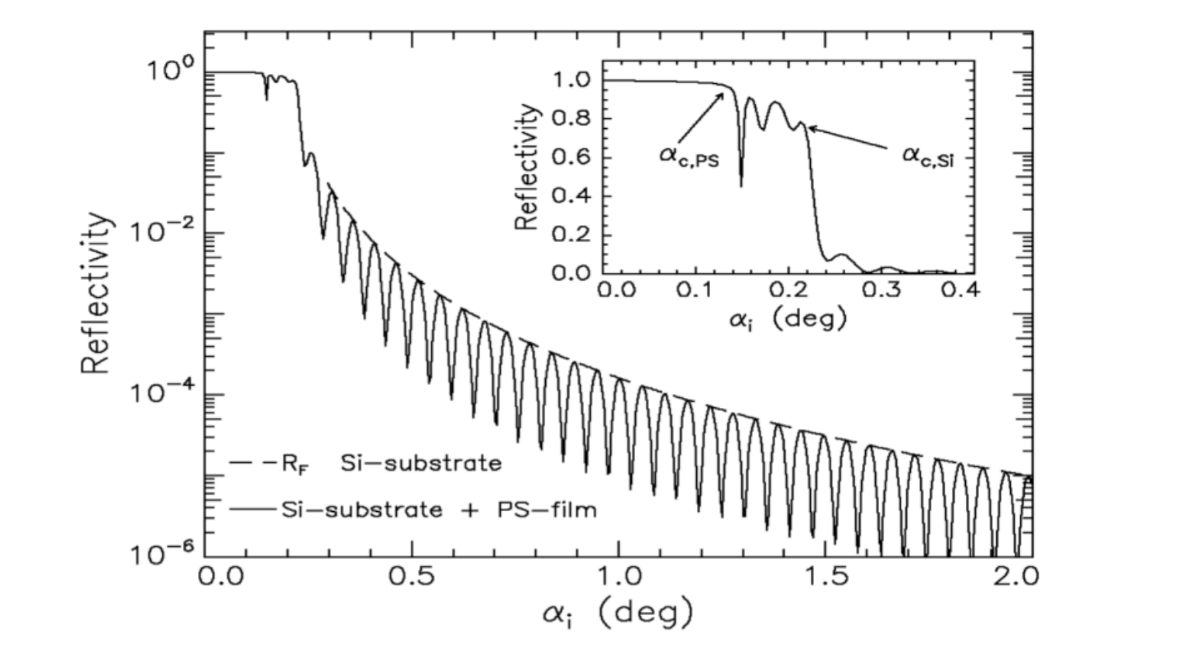
\includegraphics[scale=0.45]{images/Evtl.png}
  \caption{Die Reflektivität eines Mehrschichtsystems beispielhaft gegen den Einfallswinkel $\alpha_i$ aufgetragen.\cite{Tolan}}
  \label{fig:mss}
\end{figure}
\noindent
In dem vergrößerten Ausschnitt sind zwei Totalreflexionen zu erkennen, welche zum einen vom Siliziumsubstrat und zum anderen
vom Polystyrolfilm stammen. Oszillationen beim Abfall der Reflektivität treten auf wegen Interferenzeffekten an der Oberfläche.
Hierdurch sind Rückschlüsse auf den Schichtabstand möglich. Bei einer destruktiven Intereferenz muss ein Gangunterschied von 
einem ungeraden Vielfachen von $\frac{\lambda}{2}$ vorliegen. Es folgt

\begin{equation*}
    d = \frac{2\pi}{\delta q_z} = \frac{\lambda}{2\delta\alpha_1},
\end{equation*}
hierbei gilt $\vec{q} = \vec{k_2}-\vec{k_1}$ und $q_2 = 2k\sin{\left(\alpha_1\right)}$.\\
\noindent
Bei $N+1$ Schichten im betrachteten System kann die Reflektivität berechnet werden mir dem rekursiven Parratt-Algorithmus.
Abbildung \ref{fig:ns} zeigt ein solches System.

\begin{figure}
    \centering
    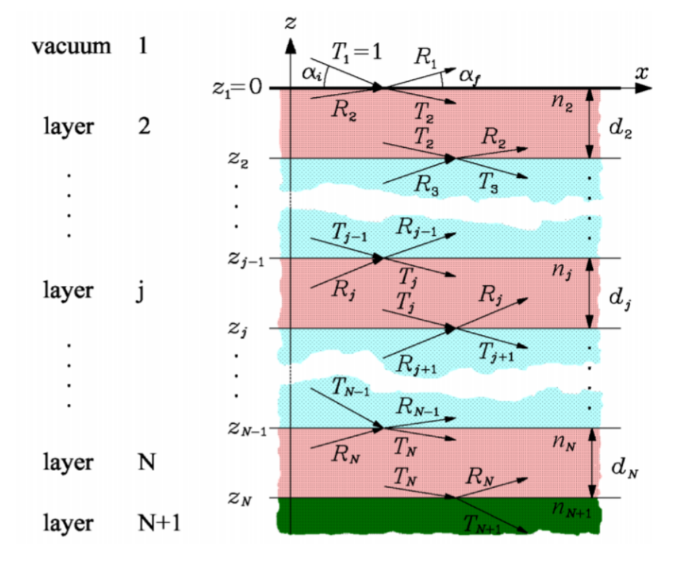
\includegraphics[scale=0.6]{images/Zwei.png}
    \caption{Eine Darstellung eines Mehrschichtsystems mit $N+1$ Schichten.\cite{Pynn}}
    \label{fig:ns}
  \end{figure}
\noindent
Die unterste Schicht ist beim Parratt-Algorithmus unendlich dick, wodurch dort keine Transmission stattfinden kann.
Die mathematische Beschreibung des Algorithmus ist

\begin{equation*}
    X_j = \frac{R_j}{T_j} = \exp{\left(-2ik_{z,j}z_j\right)}\cdot \frac{r_{j,j+1}+X_{j+1}\exp{\left(2ik_{z,j+1}z_j\right)}}{1+r_{j,j+1}X_{j+1}\exp{\left(2ik_{z,j+1}z_j\right)}}.
\end{equation*}
\noindent
$r_{j,j+1}$ beschreibt die Fresnelreflektivität an der $j$-ten Grenzfläche.
Die Startbedingung ist, dass an der untersten Schicht keine Reflextion stattfindet $R_{N+1} = 0$. Somit kann jeweils
das Verhältnis des reflektierten und transmittierten Anteils rekursiv von unten nach oben berechnet werden.

\subsection{Rauigkeit}
Die Oberfläche der Grenzfläche ist nicht perfekt glatt, was in der Berechnung der Reflektivität berücksichtigt werden muss.
Dafür werden die Fresnelkoeffizienten modifiziert zu

\begin{align*}
    \tilde{r}_{j,j+1} &= r_{j,j+1} \exp{\left(-2k_{z,j}k_{z,j+1}\sigma_j^2\right)},\\
    \tilde{t}_{j,j+1} &= t_{j,j+1} \exp{\left(\left(k_{z,j-k_{z,j+1}}\right)^2\cdot\frac{\sigma_j^2}{2}\right)}.
\end{align*}

\subsection{Geometriefaktor und Geometriewinkel}

Abbildung \ref{fig:geo} zeigt, dass der verwendete Strahl eine größere Fläche überstreicht als die Probenoberfläche. 

\begin{figure}
  \centering
  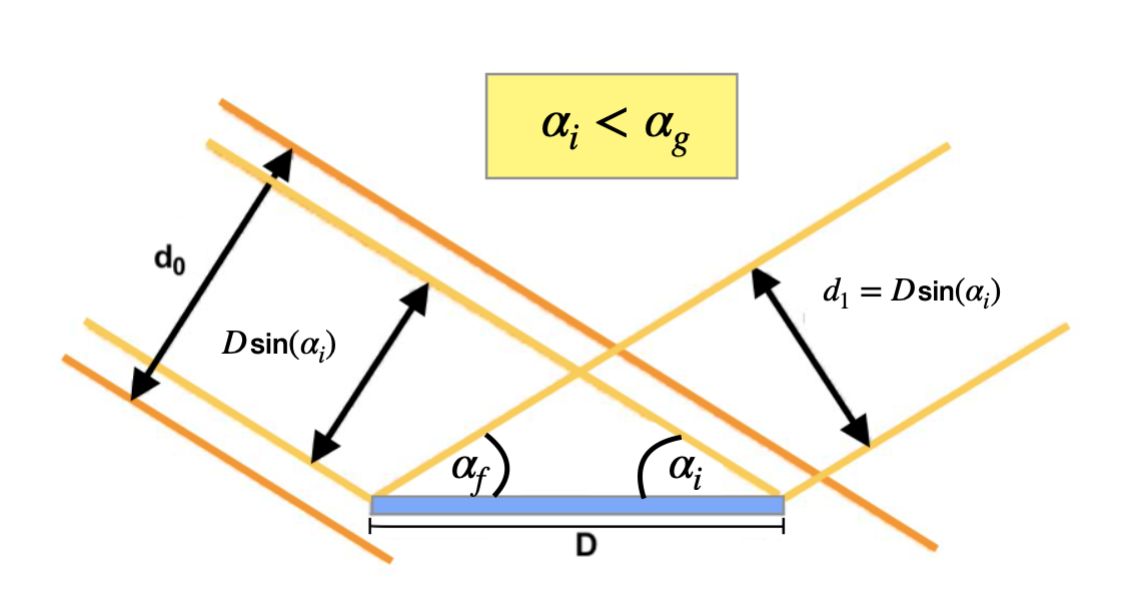
\includegraphics[scale=0.5]{images/anleit.png}
  \caption{Eine beispielhafte Veranschaulichung des Geometriewinkels. \cite{anleitung}}
  \label{fig:geo}
\end{figure} 
\noindent
Daher kann nur ein Teil der Intensität $I$ reflektiert und im Anschluss detektiert werden. Berücksichtigt wird dies
durch den Geometriefaktor $G$:

\begin{align}
    \label{eqn:geome}
    G &= \frac{D\sin{\left(\alpha_i\right)}}{d_0} \qquad &\text{mit} \qquad \alpha_i < \alpha_g,\\
    G &= 1 \qquad &\text{mit} \qquad \alpha_i > \alpha_g.
\end{align}
\noindent
Hierbei ist $D\sin{\left(\alpha_i\right)}$ die Strahlbreite, welche die Probenoberfläche trifft. $d_0$ ist die gesamte
Breite des Strahls.

\newpage
\section{Versuchsaufbau}
\label{sec:Aufbau}
Durchgeführt wird der Versuch mit einem D8-Diffraktometer.
Ein D8-Diffraktometer besteht unter Anderem aus einer Röntgenröhre mit Kupferanode. Diese wird mit einer Spannung von $\SI{40}{\kilo\volt}$ und
einer Stromstärke von $\SI{40}{\milli\ampere}$ betrieben. Die dabei entstehende Strahlung trifft auf einen Göbelspiegel, welcher die Strahlung
bündelt und monochromatisiert. Dies dient dazu, dass das nicht-polarisierte Licht, dass sich kugelförmig ausbreitet in eine
detektierbare Richtung abgelenkt wird. Der daraus resultierende Strahl besitzt eine Wellenlänge von $\lambda = \SI{1.54}{\angstrom}$.

\section{Durchführung}
\label{sec:Durchführung}
Vor der eigentlichen Messung muss der Aufbau zunächst justiert werden. 

\subsection{Justage}

Die Justage des Aufbaus erfolgt in sechs Schritten.
Als erstes wird ein Detektorscan durchgeführt, wofür die Probe nicht im Strahlgang liegt. Der Detektor und die Röntgenröhre werden auf die
Position $\SI{0}{\degree}$ gefahren. Deren Lage wird nun variiert, um die tatsächliche Nulllage des Detektors zu finden. Dies wird getan, bis die Intensität des 
Primärstrahls das Maximum durchläuft. Genau diese Position ist die normierte Nullposition. Darauf folgt der erste Z-Scan.
Hier wird die Probenjustage angepasst. Die Probe wird in den Strahlengang gebracht und die Intensität $I$ wird für verschiedene
z-Positionen gemessen. Die Position der Probe wird variiert, bis $I$ auf den Wert $I = \frac{1}{2}I_\text{max}$ sinkt. Nun misst 
man den ersten Rockingscan. Der Detektor und die Röntgenröhre werden um die Probe bewegt. Es wird ein konstanter Winkel $2\theta = \SI{0}{\degree}$ beibehalten
zwischen der Probe und dem Detektor. Das Maximum aus dem resultierenden Intensitätsverlauf wird abgelesen und für die weiteren Schritte verwendet. 
Darauf folgt der zweite Z-Scan. Weil die Position der Probe sich durch den Rockingscan verändert hat, wird ein erneuter Z-Scan durchgeführt.
Hiernach wird ein zweiter Rockingscan durchgeführt für eine Erhöhung der Präzession. Es wird erneut das Maximum abgelesen während die
Motoren entsprechend ausgerichtet werden. Als letztes wird ein dritter Rockingscan durchgeführt, bei dem mit genauerer Kalibration das
Maximum vermessen wird.

\subsection{Messung}

Nach der Justage wird ein Reflektivitätsscan durchgeführt. Der Einfallswinkel $\alpha_i$ und der Winkel zwischen Probe 
und Detektor $\alpha_\text{f}$ sind hier gleich. Es wird ein Scanbereich von $\SI{0}{\degree}$ bis $\SI{2.5}{\degree}$ und eine Schrittweite 
von $\SI{0.005}{\degree}$ gewählt. Die Messzeit beträgt $\SI{40}{\minute}$. \\
Zusätzlich wird ein diffuser Scan durchgeführt. Hier wird der Anteil der gestreuten Intensität an der Reflektivität bestimmt.

\newpage 
\printbibliography 
\end{document}